\documentclass{article}
\usepackage{amsmath}
\usepackage{graphicx}
\usepackage{MnSymbol}

\begin{document}


\title{Question 38}
\author{Ana Bhattacharjee}
\date{\today}
\maketitle{}


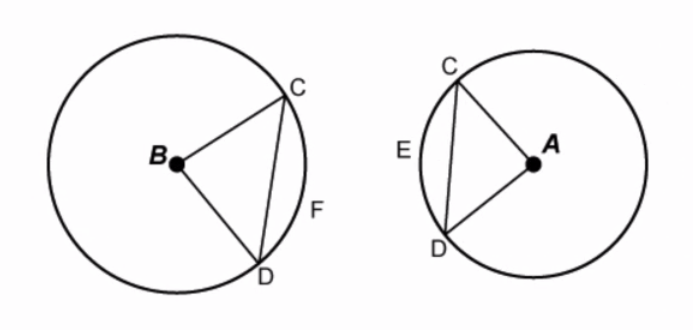
\includegraphics[width=0.9\columnwidth]{q38.png}
\paragraph{Of segments CFD and CED, which of the segments has a greater area based on the given information? Justify with your work.}
\par

\textbf{Circle A Information: }
\par
$ r = 10 m $, $ m\angle{CAD} = 90^\circ$
\par
\textbf{Circle B Information: }
\par
$ r = 12 m $, $ m\angle{CBD} = 60^\circ$

The first step is to find the area of $ \downslice CD $ for both $ \circ B $ and $ \circ A $ .

\begin{align}
  A_{\circ B} = \pi (12)^2 = 144 \pi \\
  A_{\downslice CD_{\circ B}} = \frac{60}{360} A_{\circ B} = \frac{1}{6} 144 \pi \\
  A_{\circ A} = \pi (10)^2 = 100 \pi \\
  A_{\downslice CD_{\circ A}} = \frac{90}{360} A_{\circ A} = \frac{1}{4} 100 \pi
\end{align}

\par

The next step would be to find the area of $ \triangledown{CBD} $ and $ \triangledown{CAD} $ .
\par
The new image below shows the visual explanation of why $\triangledown{CBD}$ is an equilateral triangle and $\triangledown{CAD}$ is a 45-45-90 special right triangle.
\begin{center}
  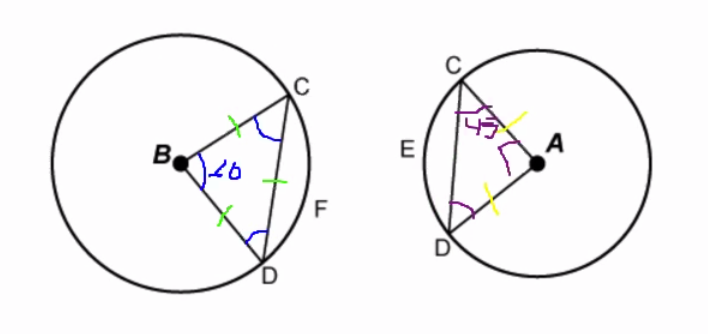
\includegraphics[width=1.1\columnwidth]{q38p2.png}
\end{center}

\par

\begin{align}
  \overleftrightarrow{CA} = 10 \\
  \overleftrightarrow{AD} = 10 \\
  \overleftrightarrow{CD} = 10 \sqrt{2} \\
  \overleftrightarrow{AE} = \sqrt{10^2 - (5\sqrt{2})^2} \\
  \overleftrightarrow{AE} = 5 \sqrt{2} = h
\end{align}
\par
\begin{align}
  A_{\triangledown{CBD}} = \frac{1}{4}(12)^2 \sqrt{3} \\
  A_{\triangledown{CBD}} = 36 \sqrt{3} \\
  A_{\triangledown{CAD}} =  \frac{1}{2} 10\sqrt{2} * 5\sqrt{2} \\
  A_{\triangledown{CAD}} = (5 \sqrt{2})^2 = 50
\end{align}

Finally, find the area of both segments $\overlinesegment{CFD}$ and $\overlinesegment{CED}$ .

\begin{align}
  \overlinesegment{CFD} = A_{\downslice CD_{\circ B}} - A_{\triangledown{CBD}} \\
  \overlinesegment{CAD} = A_{\downslice CD_{\circ A}} - A_{\triangledown{CAD}} \\
  \overlinesegment{CFD} = \frac{144 \pi}{6} - 36 \sqrt{3} \approx 13.04 \\
  \overlinesegment{CAD} = \frac{100 \pi}{4} - 50 \approx 28.54 \\
  \overlinesegment{CAD} > \overlinesegment{CFD}
\end{align}

Due to the above calculations, $\overlinesegment{CAD}$ is greater than $\overlinesegment{CFD}$.



\end{document}
